\section{Results}

\begin{figure}[h]
 \centering
 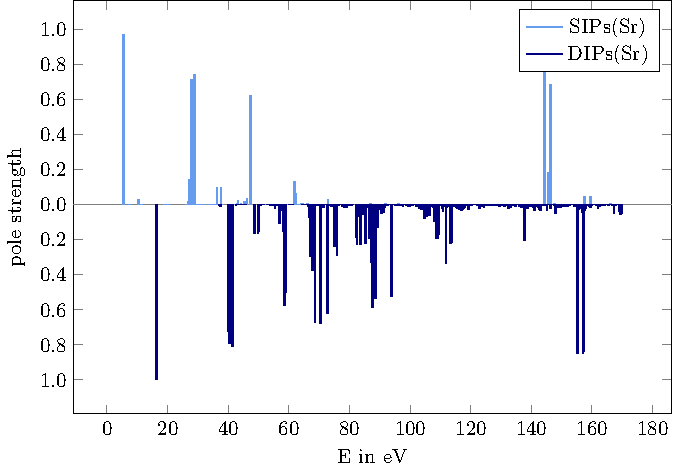
\includegraphics[width=\columnwidth]{pics/Sr_rel_sdip.pdf}
 \caption{Comparison of the single (SIP) and double (DIP) ionization spectra
          of the strontium obtained by a DC-ADC calculation.}
 \label{fig:sdip}
\end{figure}

\begin{table}[h]
 \centering
 \caption{}
 \begin{tabular}{lrrr}
  \toprule
   initial state    & energy $[\unit{eV}]$ & ps & $\Gamma [\unit{meV}]$\\
  \midrule
   Sr spinfree      & 28.599 & 0.78 &   0.56\\  
   Sr$4p_{1/2,1/2}$ & 29.402 & 0.80 &   0.10\\
   Sr$4p_{3/2,1/2}$ & 28.277 & 0.76 &   1.23\\
   Sr$4p_{3/2,3/2}$ & 28.277 & 0.76 &   1.17\\
%  \midrule
%   Ba$5p_{1/2,1/2}$ & 25.108 & 0.80 & unreliable\\
%   Ba$5p_{3/2,1/2}$ & 23.106 & 0.76 &   55.9\\
%   Ba$5p_{3/2,3/2}$ & 23.106 & 0.76 &   63.1\\
  \midrule
   Ra spinfree      & 21.836 & 0.49 &  28.56 \\  
   Ra$6p_{1/2,1/2}$ & 25.494 & 0.78 &   0.26\\
   Ra$6p_{3/2,1/2}$ & 19.267 & 0.50 &  93.16 \\
   Ra$6p_{3/2,3/2}$ & 19.267 & 0.50 &  98.86\\
  \bottomrule
 \end{tabular}
 \label{tab:widths}
\end{table}


\begin{figure}[h]
 \centering
 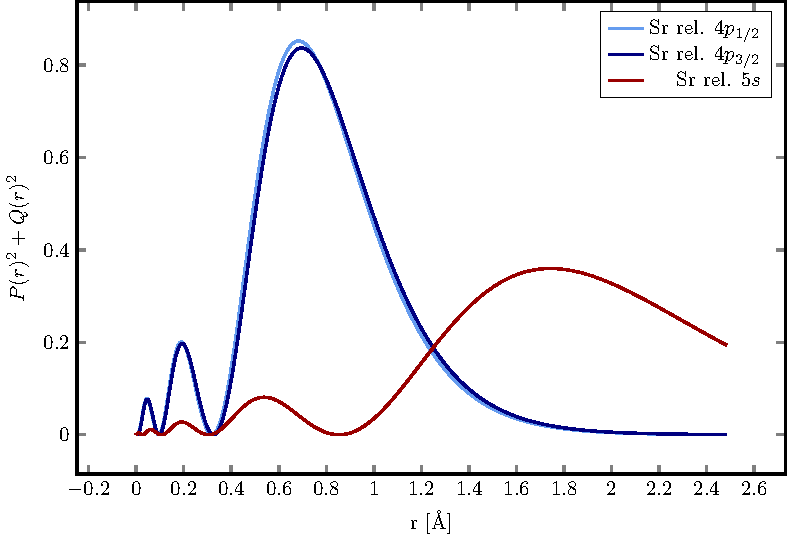
\includegraphics[width=\columnwidth]{pics/sr_ion_R.pdf}\\
 %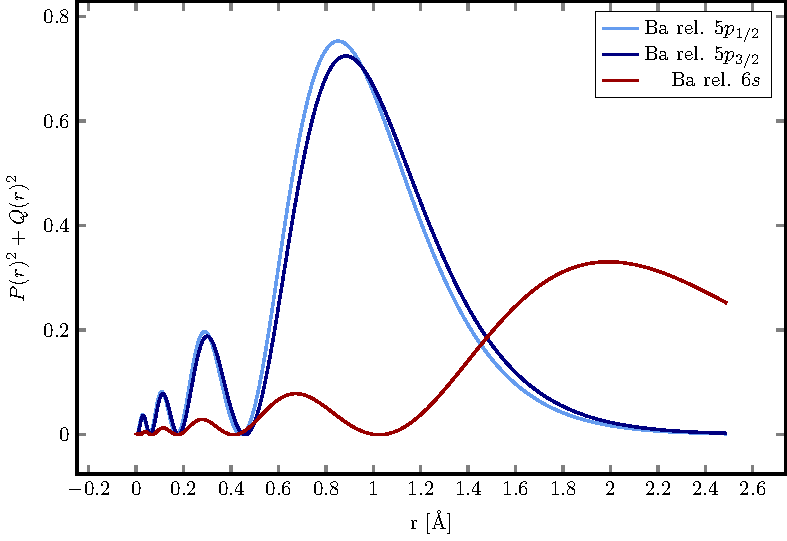
\includegraphics[width=\columnwidth]{pics/ba_ion_R.pdf}\\
 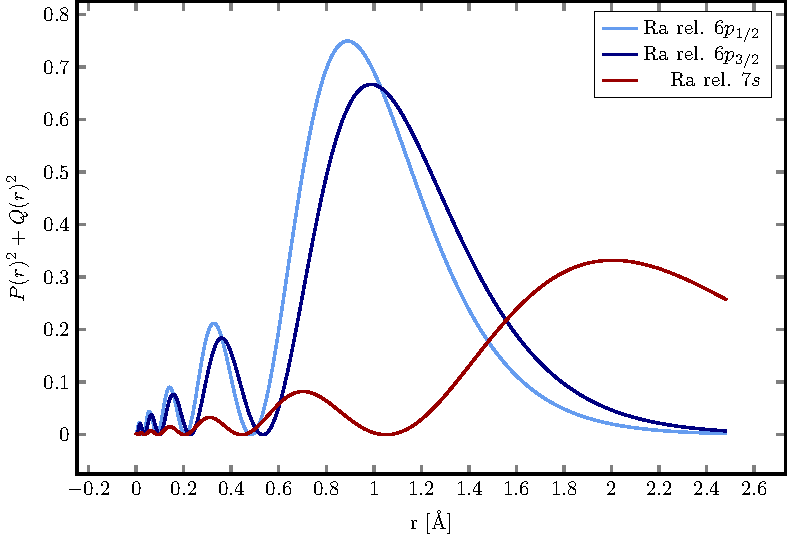
\includegraphics[width=\columnwidth]{pics/ra_ion_R.pdf}\\
 \caption{Radial densities of the orbitals of the $(n-1)p^5s^2$ ions
          involved in the Auger decay.
          The expectation value of the electrons position of the $(n-1)p_{1/2}$
          orbital is lower than of the respective $(n-1)p_{3/2}$
          orbitals. The $ns$ orbitals of the ions experience a stronger
          contraction the those of the atom (not shown here).}
 \label{fig:radial}
\end{figure}
